% Metódy inžinierskej práce

\documentclass[10pt,twoside,slovak,a4paper]{article}

\usepackage[slovak]{babel}
%\usepackage[T1]{fontenc}
\usepackage[IL2]{fontenc} % lepšia sadzba písmena Ľ než v T1
\usepackage[utf8]{inputenc}
\usepackage{graphicx}
\usepackage{url} % príkaz \url na formátovanie URL
\usepackage{hyperref} % odkazy v texte budú aktívne (pri niektorých triedach dokumentov spôsobuje posun textu)

\usepackage{cite}
%\usepackage{times}

\pagestyle{headings}

\title{Vývin inovatívnej platformy e-learningu pre nepočujúcich\thanks{Semestrálny projekt v predmete Metódy inžinierskej práce, ak. rok 2020/21, vedenie: Ing. Ján Lang, PhD.}} % meno a priezvisko vyučujúceho na cvičeniach

\author{Petra Hlavinová\\[2pt]
	{\small Slovenská technická univerzita v Bratislave}\\
	{\small Fakulta informatiky a informačných technológií}\\
	{\small \texttt{xhlavinova@stuba.sk}}
	}

\date{\small 15. október 2020} % upravte



\begin{document}

\maketitle

\begin{abstract}
E-learning je čoraz viac atraktívnejším nástrojom pre študentov. Vďaka neustálemu rozširovaniu inteligentných zariadení a modernej technológie sa stáva učenie a získavanie informácií stále jednoduchšie a rýchlejšie. Práve pre nepočujúcich študentov môže mať e-learning množstvo výhod, no napriek tomu čelí táto skupina so špecifickými vzdelávacími potrebami v dnešnej dobe mnohým prekážkam v prístupe ku vzdelávaniu. V tejto štúdii sme sa zamerali na skúmanie týchto prekážok, spôsobu, akým sa nepočujúci učia, ako aj na to, ako by im mali byť prezentované informácie a najmä vzdelávací obsah. Naším cieľom bolo analyzovať kognitívne vlastnosti nepočujúcich a hlavne nájsť a vyvinúť inovatívnu a užívateľský prívetivú platformu e-learningu vhodnú pre potreby nepočujúcich študentov. 
\end{abstract}



\section{Úvod}

Zdá sa, že nepočujúci ľudia sú v dnešnej dobe stále do veľkej miery sociálne vylúčení. Sociálne vylúčenie nepočujúcich je podmienené viacerými faktormi, či už vzdelávacím systémom, hospodárskou politikou, právnymi predpismi v sociálnej oblasti a postojmi ľudí v spoločnosti. Paradoxne však práve celoživotné vzdelávanie predstavuje rozhodujúci parameter proti sociálnemu vylúčeniu nepočujúcich ľudí. Vznik e-learningu uľahčil vzdelávanie pre ľudí na celom svete. Sila internetu, a teda aj e-learning, spočíva v jeho univerzálnosti. Z toho vyplýva, že musí byť prístupný ľuďom s rôznym rozsahom sluchu, zraku, pohybu a kognitívnych schopností.  V minulosti sa však zvyklo myslieť, že nepočujúcim stačí na uchopenie informácií písomný prepis zvukového obsahu. Práve toto predstavuje hlavný problém pri vzdelávaní tejto cieľovej skupiny, ktorému sa budeme potrebnejšie venovať v kapitole číslo ~\ref{rozdiely} .Práve preto, aby e-vzdelávanie pokrylo túto medzeru v gramotnosti, sú potrebné kreatívne spôsoby prezentácie a koordinácie interaktívnych vizuálnych materiálov.
Dôležité súvislosti sú uvedené v častiach~\ref{dolezita} a~\ref{dolezitejsia}.
Záverečné poznámky prináša časť~\ref{zaver}.



\section{Vplyv internetu na skupinu sluchovo postihnutých} \label{vplyvinternetu}

Podľa World Wide Web Consortium bol internet navrhnutý tak, aby fungoval pre všetkých jednotlivcov bez ohľadu na ich schopnosti. Vplyv internetu zásadne mení prístup k vzdelávaniu pre nepočujúcich, pretože jeho použitie odstraňuje komunikačné a interakčné bariéry, ktorým môžu jednotlivci vo fyzickom svete čeliť. To zdôrazňuje potrebu poskytnúť ľuďom so zdravotným postihnutím príležitosti bez ohľadu na ich zdravotné postihnutie sprístupnením online služieb, najmä e-learningu, spôsobom, ktorý rešpektuje a zohľadňuje ich potreby.Nejde len o rovnaké ľudské práva, ale aj o to, aby táto technológia a jej výhody mali mať úžitok aj pre nepočujúcich a sluchovo postihnutých ľudí. Inak provokuje fenomén „digitálnej priepasti“.\linebreak
Citované z \cite{pappas2018learning}
Z obr.~\ref{f:rozhod} je všetko jasné. 

\begin{figure*}[tbh]
\centering
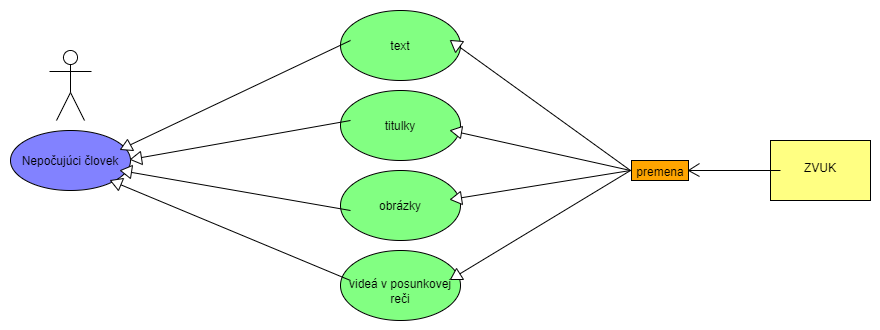
\includegraphics[scale=1.0]{diagram.pdf}
Aj text môže byť prezentovaný ako obrázok. Stane sa z neho označný plávajúci objekt. Po vytvorení diagramu zrušte znak \texttt{\%} pred príkazom \verb|\includegraphics| označte tento riadok ako komentár (tiež pomocou znaku \texttt{\%}).
\caption{Rozhodujúci argument.}
\label{f:rozhod}
\end{figure*}



\section{Iná časť} \label{ina}

Základným problémom je teda\ldots{} Najprv sa pozrieme na nejaké vysvetlenie (časť~\ref{ina:nejake}), a potom na ešte nejaké (časť~\ref{ina:nejake}).\footnote{Niekedy môžete potrebovať aj poznámku pod čiarou.}

Môže sa zdať, že problém vlastne nejestvuje\cite{Coplien:MPD}, ale bolo dokázané, že to tak nie je~\cite{Czarnecki:Staged, Czarnecki:Progress}. Napriek tomu, aj dnes na webe narazíme na všelijaké pochybné názory\cite{PLP-Framework}. Dôležité veci možno \emph{zdôrazniť kurzívou}.


\subsection{Nejaké vysvetlenie} \label{ina:nejake}

Niekedy treba uviesť zoznam:

\begin{itemize}
\item jedna vec
\item druhá vec
	\begin{itemize}
	\item x
	\item y
	\end{itemize}
\end{itemize}

Ten istý zoznam, len číslovaný:

\begin{enumerate}
\item jedna vec
\item druhá vec
	\begin{enumerate}
	\item x
	\item y
	\end{enumerate}
\end{enumerate}


\subsection{Ešte nejaké vysvetlenie} \label{ina:este}

\paragraph{Veľmi dôležitá poznámka.}
Niekedy je potrebné nadpisom označiť odsek. Text pokračuje hneď za nadpisom.



\section{Dôležitá časť} \label{dolezita}




\section{Ešte dôležitejšia časť} \label{dolezitejsia}




\section{Záver} \label{zaver} % prípadne iný variant názvu



%\acknowledgement{Ak niekomu chcete poďakovať\ldots}


% týmto sa generuje zoznam literatúry z obsahu súboru literatura.bib podľa toho, na čo sa v článku odkazujete
\bibliography{literatura}
\bibliographystyle{plain} % prípadne alpha, abbrv alebo hociktorý iný
\end{document}
